\chapter{Longitudinal stability of an aircraft}
% introduzione... stabilità, grafici e quali sono tutti i dati che servono

\section{Aerodynamic Lift}
% intro
\subsection{Wing}
\subsection{Fuselage}
\subsection{Horizontal Tail}
\subsubsection{Elevator index of effectiveness}
 In order to evaluate the contribution to the longitudinal stability of horizontal tail it's necessary to consider the deflection of the elevator. 
		
		 %disegno elevatore --> p 95 pgv
		
The variation of zero lift angle is not constant with the angle of deflection. So it's necessary to evaluate the tau factor which is defined as follows:

\begin{equation}		 
\tau_e = \frac{d \alpha_{0l}}{d \delta_e}
\end{equation}

		
Introducing this parameter the lift coefficient of the horizontal tail can be rated as follows:

\begin{equation}
C_{L_H}= C_{L_0} + C_{L_{{\alpha}_H}} \alpha_H + 	C_{L_{{\alpha}_H}} \tau_e \delta_e
\end{equation}

  
Considering a symmetrical horizontal tail, the term $C_{L_0}$ is zero, so it's possible to express the lift coefficient in the following form:


\begin{equation}
C_{L_H}= C_{L_{{\alpha}_H}} \left ( \alpha_H + \tau_e \delta_e \right)
\end{equation}
  		
 In general the value of $\tau$ is constant until about 15 deg; after this value, due to the flow separation, the effectiveness of elevator decrease and consequently the product $ \tau_e \delta_e$ that appears in the equation of lift coefficient.
		
%grafici di progetto.
		
The evaluation of tau is made by reading of external database, considering the following graphs.
	
\begin{equation}
\tau = \alpha_{\delta} \eta_{\delta} = \frac{\alpha_{{\delta}_{c_L}}}{\alpha_{{\delta}_{c_l}}}\alpha_{{\delta}_{c_l}} \eta_{\delta}
\end{equation}



%\begin{figure}[H]
%\centering
%{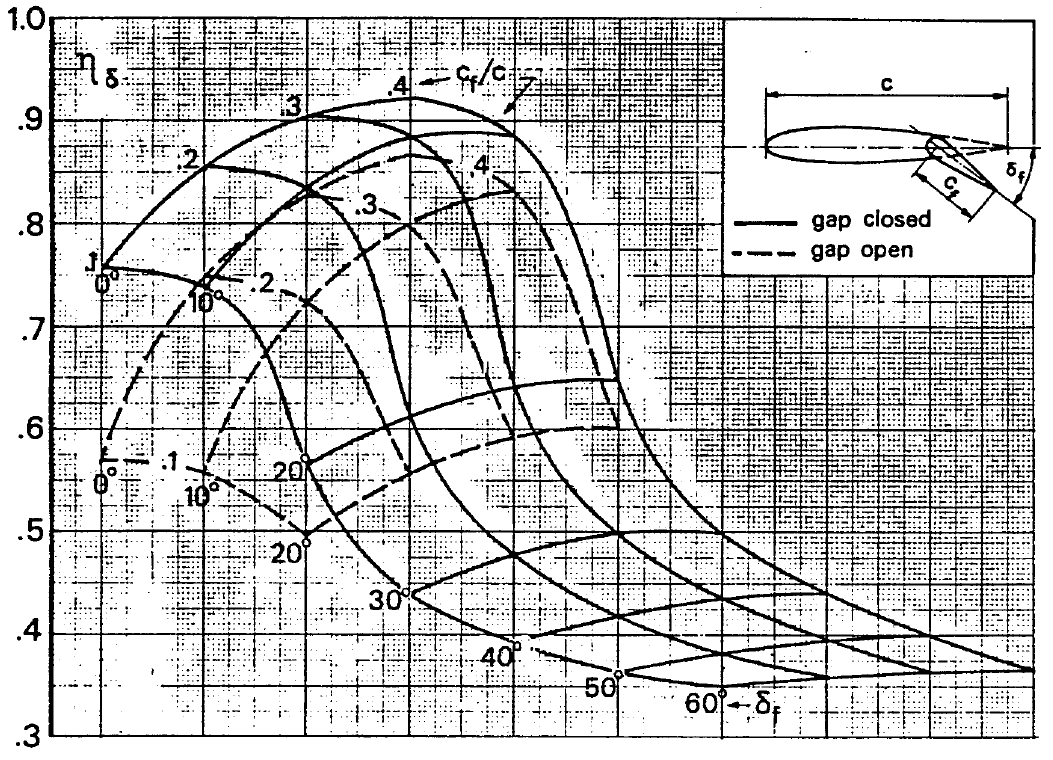
\includegraphics[height=6cm]{Immagini/Eta_Delta_Plain.png}} 
%\caption{2D efficiency correction for elevator.}
%\label{efficiency}
%\end{figure} 		
%
%
%\begin{figure}[H]
%\centering
%{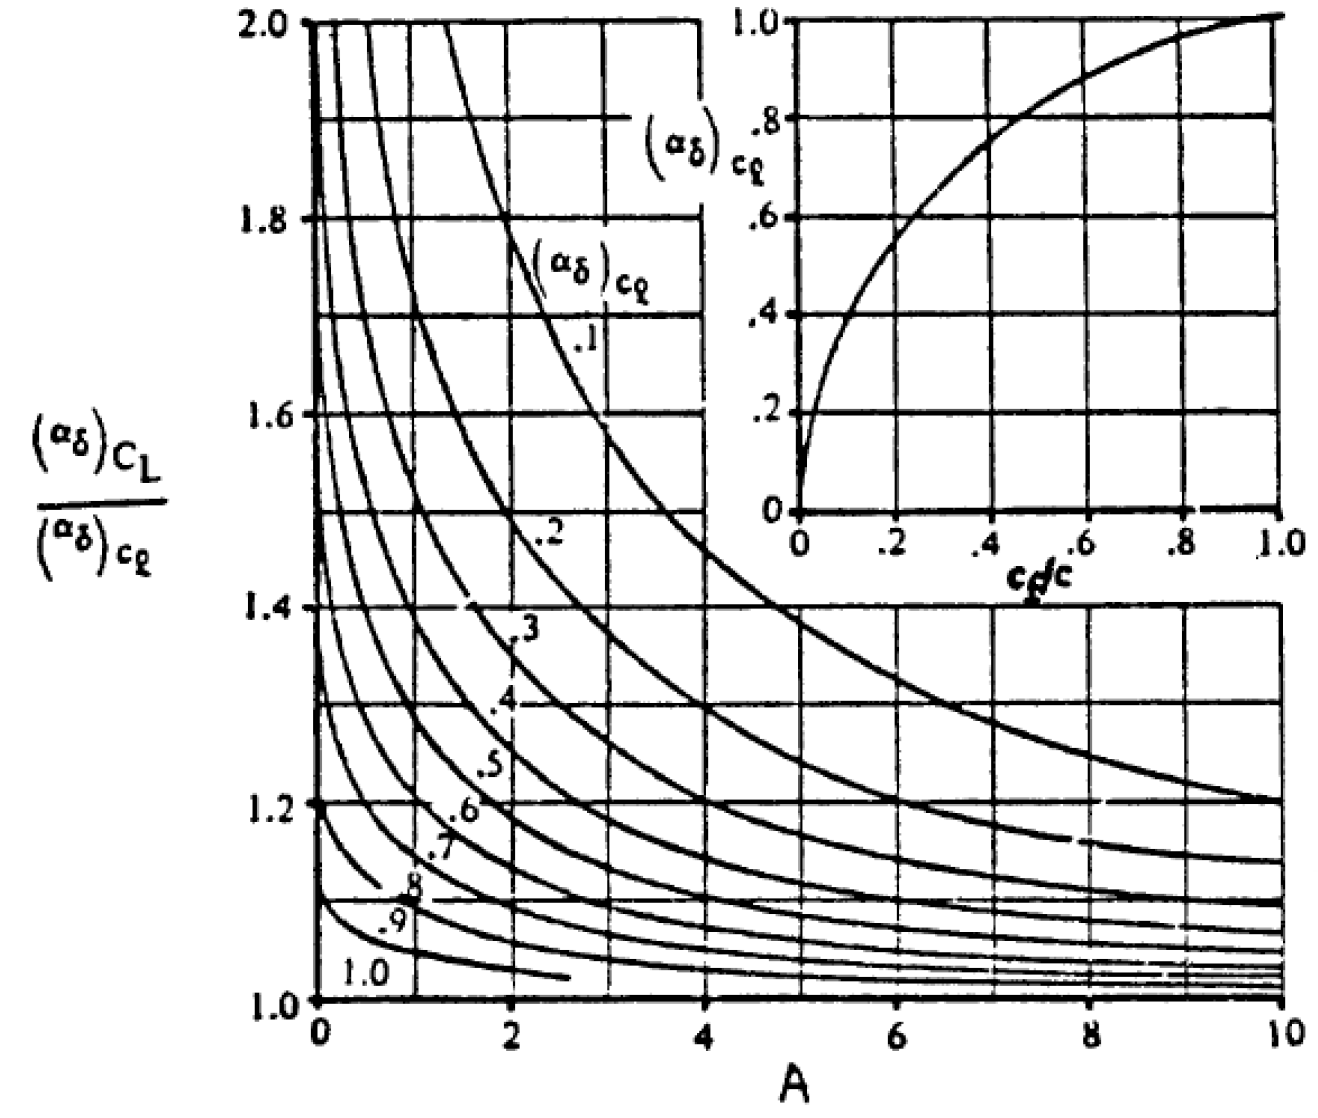
\includegraphics[height=6cm]{Immagini/alfadelta.png}} 
%\caption{$\frac{d \alpha_{0l}}{d \delta_e}$ 2D and 3D correction.}
%\label{efficiency}
%\end{figure} 		

\begin{figure}[H]
\centering
{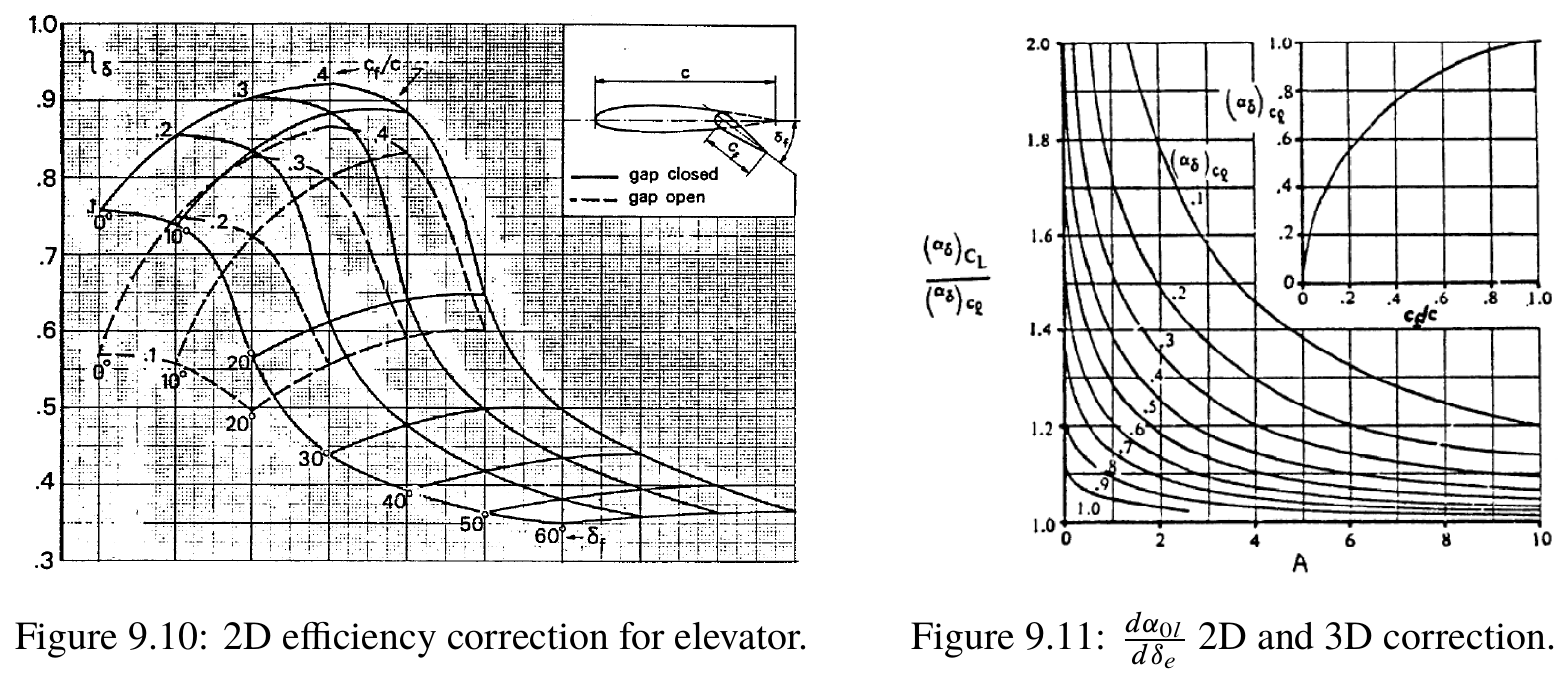
\includegraphics[height=6.79cm]{Immagini/alfadeltanew.png}} 
\label{efficiency}
\end{figure} 		


		
% java class archiecture(?)
%tabella elenco metodi con classe e che fanno

% descrizione

% spiegazione  (da fare) del calcolo del cl at alfa simile a quello dell ala
% spiegazione (da fare )  metodo calcolo tau in stability calculator
% spiegazione (gia fatta) del metodo calculateclwithdeflection in ls aerodynamic

% grafici con risultati

\subsection{Complete Aircraft}

In order to evaluate the lift coefficient of the entire airplane it's possible to consider it as consisting of the following parts\cite{ roskam2002airplane}:

\begin{itemize}
\item wing and fuselage
\item horizontal Tail
\item canard
\end{itemize}

It's important to consider the effectivness angles of attack in which the surfaces work. This is made considering the angles of incidence of the lifting surfaces and the downwash angle aft of the wing. An horizontal tail and a canard may be equiped with a trailing edge control surface. So in order to evaluate these contributes it' s important to know the angle of deflection $\delta$ of these control surfaces.\\
The calculation of the individual contributions it's reported in the relevant sections. In this section will be shown the method to evaluate the aircraft lift coefficient, known the single contributes.\\
For an aircraft with no cadard, the formula is the following:

\begin{equation}
C_L = C_{L_{wb}} + \frac{S_t}{S_w} \eta_t C_{L_{t}}
\end{equation}

Where $\eta_t$ is the ratio of dynamic pressure. In fact the dynamic pressure seen by horizontal tail differ from the free stream dynamic pressure due to two main reasons: the combination wing-fuselage and the presence of the propeller. The dynamic pressure of the tail depends on the location of the tail. If the tail is in the wake of the wing-body, the local dynamic pressure will be less than the freestream because the flow gradually looses its kinetic energy. While if the tail is in the slipstream of propeller, the local dynamic pressure may increase due to the power absorbed by the propeller.



\section{Aerodynamic Drag}

\section{Pitching Moments}
\subsection{Wing}
\subsection{Fuselage}
\subsection{Horizontal Tail}
\subsection{Propulsors}

\subsection{Stability Calculation}

% calcolo delle forze normali e tangenziali, calcolo momenti, risultati

\section{Java Class Architecture}
% intro
% riepilogo di tutte le classi in schema. vedi su quaderno  prima di stabilita
% schema in yed

\section{User's Guide}
%intro
% test class

\section{Analysis Results} % fai qui? oppure durante?
%grafici